% !TEX encoding = UTF-8 Unicode
% This is based on the LLNCS.DEM the demonstration file of
% the LaTeX macro package from Springer-Verlag
% for Lecture Notes in Computer Science,
% version 2.4 for LaTeX2e as of 16. April 2010
%
% See http://www.springer.com/computer/lncs/lncs+authors?SGWID=0-40209-0-0-0
% for the full guidelines.
%

\documentclass{llncs}
\usepackage[utf8]{inputenc}
\usepackage{graphicx}


\begin{document}

\title{Programación Genética Inductiva, un acercamiento práctico usando el lenguaje Funico}
%
\titlerunning{Programación Genética Inductiva}  % abbreviated title (for running head)
%                                     also used for the TOC unless
%                                     \toctitle is used
%
\author{Juan Pablo Salamanca Ramírez}
%
\authorrunning{Juan P. Salamanca} % abbreviated author list (for running head)
%
%%%% list of authors for the TOC (use if author list has to be modified)
\tocauthor{}
%
\institute{Departamento de Ingenieria de Sistemas e Industrial, Universidad Nacional de Colombia, Bogotá, Carrera 45 No 26-85, Colombia,\\
\email{jpsalamarcara@unal.edu.co}}

\maketitle

\begin{abstract}
Genetic programming is a research field of evolutionary computing, in which, by using genetic algorithms, is intended to optimize a population of individuals belonging to the domain of any programming language, this is done according to a certain fitness function.
In this paper, an experimental study of the different evolutionary strategies that can be adopted to apply genetic programming in the domain of Funico functional programming language occurs.
\keywords{evolutionary computation, genetic programing, inductive, functional}
\end{abstract}
%



\section{Introducción}
La programación genética es un campo de investigación de la computación evolutiva, en el cual, mediante el uso de algoritmos genéticos, se pretende optimizar una población de individuos pertenecientes al dominio de algún lenguaje de programación, esto se hace de acuerdo a una determinada función de aptitud.
En este documento, se presenta un estudio experimental acerca de las diferentes estrategias evolutivas que se pueden adoptar para aplicar la programación genética particularmente en el dominio del lenguaje de programación funcional Funico \cite{cub:gom}, desarrollado por E. Cubides.

%Fin de la Introducción
\section{Estado del Arte}
Desde las primeras propuestas hechas por Koza \cite{koza}, se han presentado continuos avances \cite{koza:1} en materia de programación genética. En el caso de la programación genética inductiva, recientemente han surgido aplicaciones que tratan problemas específicos, como por ejemplo, la detección de reglas de asociación difusas \cite{gonz} y el diseño de motores \cite{karim}.
Por otra parte, con la introducción del algoritmo HaEA \cite{gomez} en la programación genética inductiva \cite{cub:gom:2}, se permitió un gran desarrollo debido a su gran capacidad de optimización y carencia de parámetros para ajustar. Los resultados pronto serán publicados y se espera que a partir de; se descubran nuevas técnicas y mejoras en los distintos campos de aplicación.

\section{Propuesta}
Teniendo en cuenta las principales conclusiones de J. Gómez \cite{gomez} en relación a la preservación de la diversidad como estrategia evolutiva y al análisis de los diferentes esquemas de selección realizado por T. Blicke \& L. Thiele\cite{blick:thiele}; se plantea encontrar un método para seleccionar individuos de la población, en el cual se favorezca la   exploración y explotación como principios básicos para disminuir la perdida de diversidad y la probabilidad de estancamiento en un mínimo/máximo local. El resultado es un híbrido entre selección por ruleta y selección por ranking.

\subsection{Estrategia de Selección: Ruleta-Ranking}
El procedimiento de selección propuesto, llamado inicialmente Ruleta-Ranking, se describe paso a paso a continuación:
\begin{enumerate}
\item Se normalizan las medidas de aptitud de cada individuo de la población usando escala decimal.
\item Se normalizan los datos del paso anterior en el intervalo $[0,1]$
\item Se ordenan de forma descendente los individuos de acuerdo su medida de aptitud normalizada, de manera que el mejor individuo sea el primero de la lista y el peor el último.
\item Generar un número aleatorio usando una distribución normal con $\mu=0$ y $\sigma=\frac{1}{3}$, y aplicarle la función valor absoluto.
\item Seleccionar el individuo con la medida de aptitud normalizada inmediatamente mayor al número aleatorio generado en el paso anterior.
\item Retirar al individuo seleccionado de la lista y ajustar las probabilidades de los individuos restantes.
\end{enumerate}
En esta estrategia, los mejores individuos tienen mayor probabilidad de ser seleccionados inicialmente, sin embargo, con su salida de la lista de espera, se redistribuye la probabilidad en los individuos restantes, ofreciéndole prioridad a los nuevos mejores. Esta técnica permite exploración ya que por la forma de la distribución normal, existe la probabilidad de seleccionar individuos no tan buenos. Y permite explotación, porque se seleccionan los mejores en mayor proporción. 
Para controlar la complejidad del algoritmo, se mantiene la sumatoria total de las medidas de aptitud normalizadas de los individuos en espera y cada vez que alguno es elegido, su medida de aptitud es restada del total y se aplica otra normalización respecto a este nuevo total.

\paragraph{Comentario.}
Al cambiar la forma de la distribución del número generado en el paso $4$, por una con $\mu=1$, se obtiene que la ejecución del algoritmo genético minimiza la función de aptitud.

\subsection{Estrategia de Generación y Reemplazo}
Para la generación de nuevos individuos se propone como estrategia el matrimonio, generando de a dos hijos por pareja. Sin embargo, el criterio de selección de pareja se dividió en dos: por similitud y por mejor medida de aptitud, teniendo en cuenta que el mejor individuo tiene $n-1$ oportunidades de elegir, el segundo mejor individuo tiene $n-2$ y así sucesivamente hasta que el penúltimo individuo solo pudiese elegir al peor ($n$ es el tamaño total de los individuos elegibles).

Como estrategia de reemplazo se propuso estado estable y reemplazo generacional, en combinación con alguna de las estrategias de generación anteriormente descritas.

\subsection{Función de Aptitud}
Para la función de aptitud, como el resultado de cada programa en Funico es una predicción con relación a un modelo funcional interno (conjunto de ecuaciones), se propuso contar el número de aciertos por cada individuo (programa) de la población de acuerdo a un conjunto de consultas de entrenamiento y verificación que son fijadas como parámetros. Normalizando respecto al total de consultas de entrenamiento. Ademas se penaliza a aquellos individuos que presenten problemas léxicos, sintácticos y de ejecución.
\subsection{Inicialización}
Para la inicialización se tomó como base el conjunto de consultas de entrenamiento, y a partir de estas se construyen arboles completos según la estructura sintáctica de Funico. Los programas pueden tener un número de ecuaciones fijo o variable, sin embargo, este siempre debe ser mayor de 2.

\subsection{Operadores}
En cuanto a los operadores, se propone el uso de un operador de cruce y cuatro de mutación, estos últimos siguiendo un esquema de auto adaptabilidad similar al de HaEA \cite{gomez}. En la inicialización se fija una probabilidad de 0.5 por cada operador de mutación, y de acuerdo a las veces que el operador es ejecutado, se determina si aportó a la mejora de la medida de aptitud del individuo ó no; de acuerdo a esto se premia o se castiga, aumentando o disminuyendo la probabilidad de ser elegido nuevamente para ese individuo particular. Teniendo en cuenta que muchas veces un operador puede ser castigado, causando un incremento en la probabilidad de estancar la búsqueda en un máximo (ó mínimo) local, se introduce un reinicio de las probabilidades de todos lo operadores de mutación para un individuo particular, este reinicio es un proceso estocástico que sigue una distribución de probabilidad binomial con $p$ fijado como parámetro de entrada.
\subsubsection{Cruce}
El operador de cruce corresponde al operador GlobalCrossover propuesto por E. Cubides \cite{cub:gom:2}, en el cual dos  nodos principales (ecuaciones en Funico) seleccionados aleatoriamente, de dos individuos (programas) distintos son intercambiados.
\subsubsection{Mutación}
Para la mutación, se propone el uso de tres de los operadores propuestos por E. Cubides \cite{cub:gom:2}: GlobalSwap, InternalSwap y Equalization. Adicionalmente, conociendo la naturaleza del proceso de inicialización, el cual, genera individuos de un tamaño fijo (numero de ecuaciones fijo), se propone un nuevo operador: DropEquation, en el cual, uno de los arboles principales del programa (ecuación en Funico) es eliminado, para reducir la complejidad del individuo y permitir la exploración en individuos con un número de ecuaciones inferior al máximo permitido.

\section{Experimentos y Resultados}
Para el calculo de la función de aptitud, se probaron estrategias alternativas como penalización por malos patrones, tiempo de procesamiento consumido y cantidad de ecuaciones, sin embargo, los resultados no fueron favorables y se descartaron. Aunque, la penalización por problemas léxicos, sintácticos y de ejecución se mantuvo.

En el caso de la inicialización se intentó generar programas de tamaño aleatorio, respetando un mínimo de dos ecuaciones y un máximo fijado como parámetro. Pero debido a los malos resultados se optó por dejar el número de ecuaciones fijo y confiar en el operador DropEquation para obtener individuos de tamaño menor al máximo.
\subsection{Ejecución}
Para la ejecución de las diferentes estrategias se utilizó un mismo conjunto de consultas, cuyo objetivo, es hallar una expresión en Funico para calcular el módulo 3 (mod3(N)) de un número entero.
El tamaño de la población es de 100, el total de iteraciones es de 1000, el máximo número de ecuaciones por individuo es de 6, la profundidad de cada individuo en la inicialización es de 3 y el parámetro $p$ para el reinicio de las probabilidades de selección de un operador de mutación fue fijado en $0.1$ .
En \ref{Ejecucion_1} se muestran las medidas estadísticas del resultado de una ejecución, aplicando la estrategia de generación por mejor aptitud y reemplazo generacional. En \ref{Ejecucion_2} , se presentan las medidas resultado de aplicar generación por mejor aptitud y reemplazo de estado estable. La implementación de este algoritmo se puede encontrar como un archivo anexo a este, esta implmentación fue realizada completamente desde cero en lenguaje JAVA, a excepción de la librería de Funico, la cual fue proporcionada por el autor-\cite{cub:gom}. La clase que contiene el método de ejecución principal es jp.methods.gp.TestFunico.java .

\paragraph{Aclaración.}
Las estrategias de generación por similitud aunque fueron implementadas y ejecutadas, no se estudiaron con más detalle debido a su baja tasa de convergencia. De alrededor de 20 experimentos de 1000 iteraciones, en ningún momento encontró al menos un individuo solución (Individuo con aptitud 1.0)

\begin{figure}
  \centering
    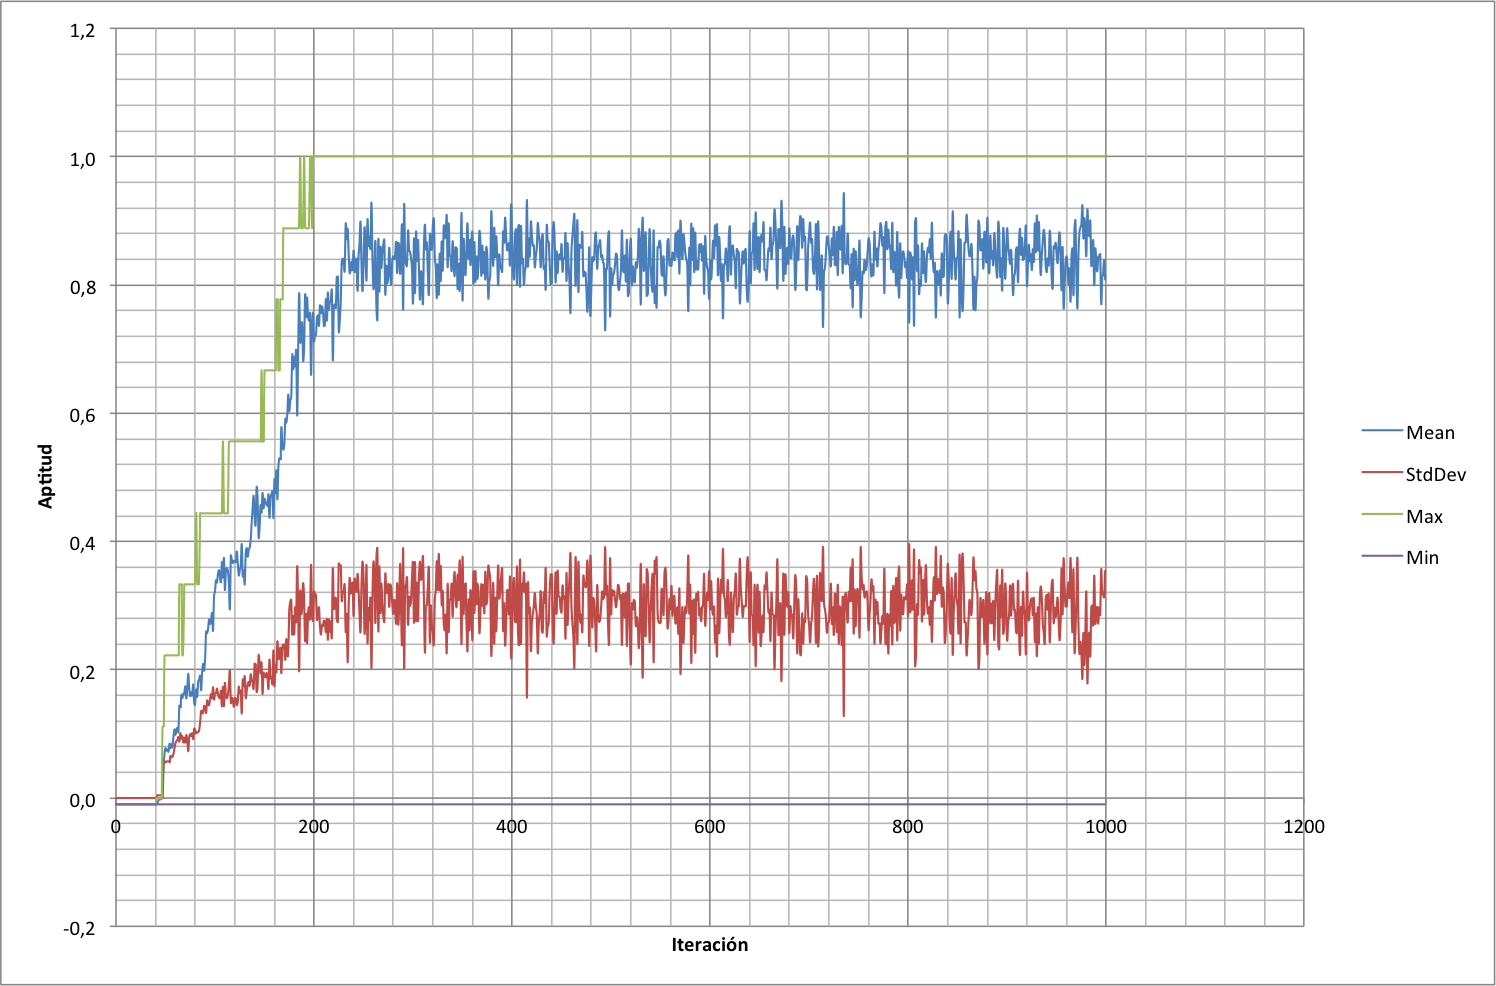
\includegraphics[width=0.95\textwidth]{GPBestFitGen}
  \caption{Generación por Mejor Aptitud  y Reemplazo Generacional}
  \label{Ejecucion_1}
\end{figure}


\begin{figure}
  \centering
    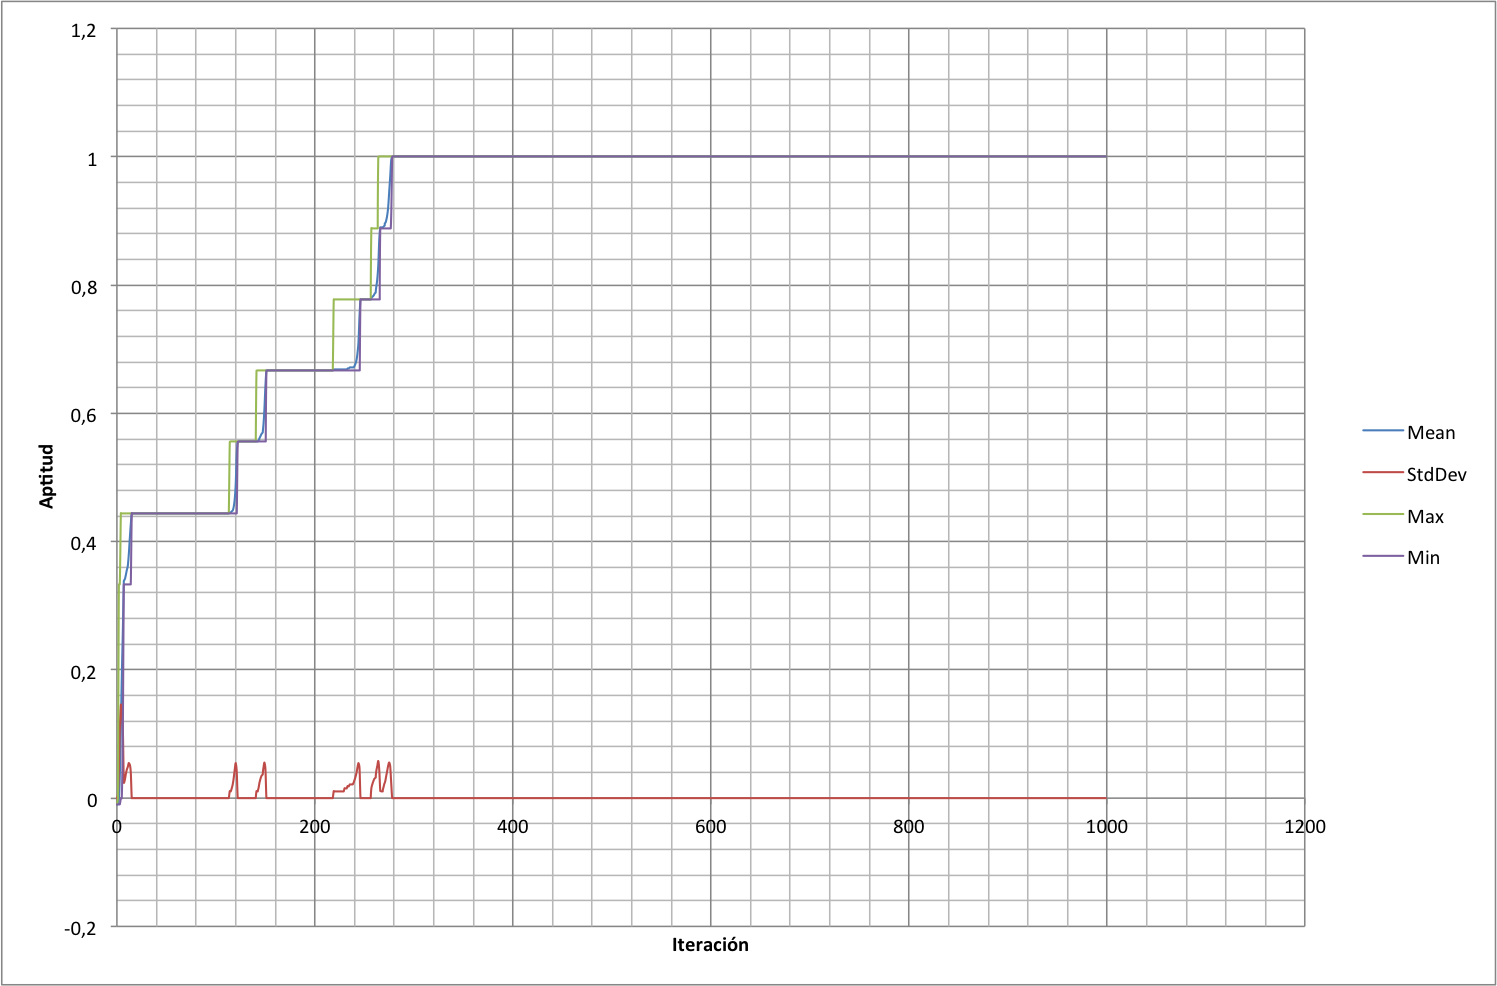
\includegraphics[width=0.95\textwidth]{GPBestFitSteady}
  \caption{Generación por Mejor Aptitud  y Reemplazo de Estado Estable}
  \label{Ejecucion_2}
\end{figure}


\section{Conclusiones}

\begin{itemize}
\item Una estrategia de reemplazo poblacional de estado estable, aumenta considerablemente la probabilidad de hallar individuos solución en el dominio de la programación genética.
\item La correcta combinación entre el proceso de generación de la población inicial y el esquema de exploración,  pueden mejorar o empeorar la velocidad de convergencia del algoritmo genético, entonces, estás estrategias deben ser planteadas de acuerdo al dominio del espacio de busqueda.
\item En el campo de la inteligencia artificial, la programación genética inductiva, puede considerarse una técnica para emular la creatividad y el pensamiento inductivo, sin embargo, su alcance puede extenderse de acuerdo a la naturaleza del lenguaje base.
\end{itemize}

\begin{thebibliography}{8}
%
\bibitem {cub:gom}
Edwin, C., Cubides, G. \& Jonatan Gómez P.:
Curso de Computación Evolutiva. Programación Funcional con el Lenguaje Funico.
Bogotá (2015)

\bibitem {koza}
Jhon R., Koza.:
Dynamic, Genetic and Chaotic Programming,
Jhon Wiley and Sons, Inc (1992)

\bibitem {koza:1}
Jhon R., Koza. et al:
Advances in Genetic Programming, 
The MIT Press, ISBN0-262-11188-8 (1994)

\bibitem {gonz}
Antonio, G. et al:
An efficient Inductive Genetic Learning Algorithm for Fuzzy Relational Rules.
International Journal of Computational Intelligence Systems, (2012)

\bibitem {karim}
S, Karim Tanatabaei et al:
Self-adjusting multidisciplinary design of hydraulic engine mount using bond graphs and inductive genetic programming.
Science Direct, (2016)

\bibitem {gomez}
J. Gómez:
Self Adaptation of Operator Rates in Evolutionary Algorithms
Universidad Nacional de Colombia and The University of Memphis, (2004)

\bibitem {cub:gom:2}
Edwin, C., Cubides, G. \& Jonatan Gómez P.:
Curso de Computación Evolutiva. Programación Genética Funcional Inductiva con el Lenguaje Funico.
Bogotá (2015)

\bibitem {blick:thiele}
Tobias Blickle \& Lothar Thiele:
A Comparison of Selection Schemes used in Genetic Algorithms.
Computer Engineering and Communication Networks Lab.
Swiss Federal Institute of Technology. (1995)

\end{thebibliography}

\end{document}

